\newpage
\section{Auswertung}

    \subsection{Überprüfung der Bragg-Bedingung}

        \noindent Die Bragg-Bedingung wird überprüft indem der LiF-Kristall auf einen festen Winkel $\theta = \SI{14}{\degree}$ gestellt und der Winkel
        $\alpha$ des Geiger-Müller-Zählrohrs von $\SI{26}{\degree}$ bis $\SI{30}{\degree}$ in $\increment \alpha = \SI{0.1}{\degree}$ Schritten 
        verändert.\\ Auf jeden dieser Schritte werden für $t = 5s$ die Anschläge gemessen. Die Daten zu dieser Messung sind in Tabelle(\ref{tab:Bragg}) 
        zu finden.

        \begin{table}
            \centering
            \caption{Die Messwerte von der Überprüfung der Bragg-Bedingung.}
            \label{tab:Bragg}
            \begin{tabular}{S[table-format=2.1] S[table-format=3.1] S[table-format=2.1] S[table-format=3.1]}
              \toprule
              $\alpha_{\text{GM}} \mathbin{/} \si{\degree}$ & $ N \mathbin{/} \si{Imp\per\second}$ &
              $\alpha_{\text{GM}} \mathbin{/} \si{\degree}$ & $ N \mathbin{/} \si{Imp\per\second}$ \\
              %$\alpha_{\text{GM}} \, \mathbin{/} \si{\degree}$ & $ N \, [\text{Imp}/ \si{\second}$ & 
              %$\alpha_{\text{GM}} \, \mathbin{/} \si{\degree}$ & $ N \, [\text{Imp}/ \si{\second}$ \\
              \midrule
              26.0 &	56.0  &    28.1 &	215.0 \\
              26.1 &	58.0  &    28.2 &	218.0 \\
              26.2 &	54.0  &    28.3 &	215.0 \\
              26.3 &	62.0  &    28.4	& 208.0 \\
              26.4 &	58.0  &    28.5	& 189.0 \\
              26.5 &	68.0  &    28.6	& 189.0 \\
              26.6 &	72.0  &    28.7	& 176.0 \\
              26.7 &	83.0  &    28.8	& 164.0 \\
              26.8 &	89.0  &    28.9	& 149.0 \\
              26.9 &	95.0  &    29.0	& 138.0 \\
              27.0 &	105.0 &    29.1	& 125.0 \\
              27.1 &	119.0 &    29.2	& 111.0 \\
              27.2 &	125.0 &    29.3	& 107.0 \\
              27.3 &	141.0 &    29.4	& 95.0  \\
              27.4 &	154.0 &    29.5	& 77.0  \\
              27.5 &	157.0 &    29.6	& 73.0  \\
              27.6 &	166.0 &    29.7	& 58.0  \\
              27.7 &	180.0 &    29.8	& 56.0  \\
              27.8 &	188.0 &    29.9	& 53.0  \\
              27.9 &	211.0 &    30.0	& 53.0  \\
              28.0 &	212.0 \\
              \bottomrule
            \end{tabular}
          \end{table}

          \noindent Diese Daten sind in Plot(\ref{fig:bragg}) dargestellt und der Punkt mit den meisten Anschlägen bei $\alpha = \SI{28.2}{\degree}$ markiert. 
          Der theoretische Sollwinkel liegt nach dem Reflexionsgestz bei $\alpha = \SI{28}{\degree}$. Es liegt also nur eine Abweichung von 
          $\SI{0.7}{\percent}$ vor.

          \begin{figure}
            \centering
            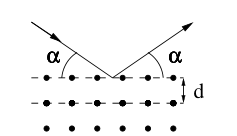
\includegraphics[width=\textwidth]{build/plots/Bragg.pdf}
            \caption{Die Messreihe zur Überprüfung der Bragg-Bedingung aufgetragen in einem $\alpha$ - $N$- Diagramm.}
            \label{fig:bragg}
          \end{figure}

    \subsection{Emissionsspektrums der Cu-Röntgenröhre}\label{sec:Cu-Röntgenröhre}

         
        \noindent Zur Analyse des Emissionsspektrums der Cu-Röntgenröhre werde die Anschläge des Zählrohrs in 10 Sekunden Intervallen mit 
        Schrittlängen von $\Delta \theta = \SI{0.1}{\degree}$ gemessen. Diese Messwerte sind in Tabelle(\ref{tab:emissionsspektrum}) dargestellt.
        
        \begin{table}
            \centering
            \caption{Die Messwerte des Emissionsspektrum der Kupfer-Röntgenröhre.}
            \label{tab:emissionsspektrum}
            \begin{tabular}{S[table-format=2.1] S[table-format=3.1] S[table-format=2.1] S[table-format=3.1] S[table-format=2.1] S[table-format=3.1] S[table-format=2.1] S[table-format=4.1] S[table-format=2.1] S[table-format=4.1]}
              \toprule
              $ \theta \, \mathbin{/} \si{\degree}$ & $ N \, \mathbin{/} \si{Imp\per\second}$ & 
              $ \theta \, \mathbin{/} \si{\degree}$ & $ N \, \mathbin{/} \si{Imp\per\second}$ &
              $ \theta \, \mathbin{/} \si{\degree}$ & $ N \, \mathbin{/} \si{Imp\per\second}$ &
              $ \theta \, \mathbin{/} \si{\degree}$ & $ N \, \mathbin{/} \si{Imp\per\second}$ &
              $ \theta \, \mathbin{/} \si{\degree}$ & $ N \, \mathbin{/} \si{Imp\per\second}$ \\
              \midrule
              8.0 	&	323.0 &    11.5	&	406.0 &    14.9	&	248.0 &     18.3	&	166.0  &      21.7	&	164.0 \\   
              8.1 	&	316.0 &    11.6	&	404.0 &    15.0	&	253.0 &     18.4	&	173.0  &      21.8	&	180.0 \\   
              8.2 	&	326.0 &    11.7	&	405.0 &    15.1	&	257.0 &     18.5	&	167.0  &      21.9	&	179.0 \\   
              8.3 	&	340.0 &    11.8	&	400.0 &    15.2	&	248.0 &     18.6	&	169.0  &      22.0	&	191.0 \\   
              8.4 	&	335.0 &    11.9	&	383.0 &    15.3	&	242.0 &     18.7	&	160.0  &      22.1	&	232.0 \\   
              8.5 	&	343.0 &    12.0	&	389.0 &    15.4	&	249.0 &     18.8	&	159.0  &      22.2	&	300.0 \\   
              8.6 	&	350.0 &    12.1	&	382.0 &    15.5	&	246.0 &     18.9	&	157.0  &      22.3	&	536.0 \\   
              8.7 	&	350.0 &    12.2	&	372.0 &    15.6	&	252.0 &     19.0	&	149.0  &      22.4	&	4128.0\\    
              8.8 	&	366.0 &    12.3	&	376.0 &    15.7	&	236.0 &     19.1	&	153.0  &      22.5	&	5050.0\\    
              8.9 	&	357.0 &    12.4	&	385.0 &    15.8	&	234.0 &     19.2	&	150.0  &      22.6	&	4750.0\\    
              9.0 	&	371.0 &    12.5	&	384.0 &    15.9	&	231.0 &     19.3	&	147.0  &      22.7	&	4571.0\\    
              9.1 	&	371.0 &    12.6	&	382.0 &    16.0	&	215.0 &     19.4	&	150.0  &      22.8	&	4097.0\\    
              9.2 	&	372.0 &    12.7	&	373.0 &    16.1	&	217.0 &     19.5	&	148.0  &      22.9	&	901.0 \\   
              9.3 	&	364.0 &    12.8	&	376.0 &    16.2	&	227.0 &     19.6	&	149.0  &      23.0	&	244.0 \\   
              9.4 	&	381.0 &    12.9	&	373.0 &    16.3	&	214.0 &     19.7	&	143.0  &      23.1	&	179.0 \\   
              9.5 	&	379.0 &    13.0	&	375.0 &    16.4	&	217.0 &     19.8	&	153.0  &      23.2	&	151.0 \\   
              9.6 	&	393.0 &    13.1	&	366.0 &    16.5	&	210.0 &     19.9	&	182.0  &      23.3	&	145.0 \\   
              9.7 	&	375.0 &    13.2	&	354.0 &    16.6	&	211.0 &     20.0	&	291.0  &      23.4	&	130.0 \\   
              9.8 	&	391.0 &    13.3	&	341.0 &    16.7	&	206.0 &     20.1	&	1127.0 &      23.5	&	121.0 \\    
              9.9 	&	395.0 &    13.4	&	326.0 &    16.8	&	205.0 &     20.2	&	1599.0 &      23.6	&	126.0 \\    
              10.0	&	402.0 &    13.5	&	318.0 &    16.9	&	198.0 &     20.3	&	1533.0 &      23.7	&	117.0 \\    
              10.1	&	405.0 &    13.6	&	305.0 &    17.0	&	203.0 &     20.4	&	1430.0 &      23.8	&	112.0 \\    
              10.2	&	390.0 &    13.7	&	296.0 &    17.1	&	199.0 &     20.5	&	1267.0 &      23.9	&	110.0 \\    
              10.3	&	398.0 &    13.8	&	286.0 &    17.2	&	198.0 &     20.6	&	425.0  &      24.0	&	105.0 \\   
              10.4	&	400.0 &    13.9	&	285.0 &    17.3	&	191.0 &     20.7	&	241.0  &      24.1	&	106.0 \\   
              10.5	&	418.0 &    14.0	&	274.0 &    17.4	&	192.0 &     20.8	&	225.0  &      24.2	&	107.0 \\   
              10.6	&	401.0 &    14.1	&	264.0 &    17.5	&	184.0 &     20.9	&	192.0  &      24.3	&	95.0  \\  
              10.7	&	410.0 &    14.2	&	266.0 &    17.6	&	191.0 &     21.0	&	188.0  &      24.4	&	94.0  \\  
              10.8	&	408.0 &    14.3	&	270.0 &    17.7	&	188.0 &     21.1	&	172.0  &      24.5	&	100.0 \\   
              10.9	&	409.0 &    14.4	&	255.0 &    17.8	&	181.0 &     21.2	&	168.0  &      24.6	&	91.0  \\  
              11.0	&	414.0 &    14.5	&	255.0 &    17.9	&	185.0 &     21.3	&	169.0  &      24.7	&	85.0  \\  
              11.1	&	420.0 &    14.6	&	260.0 &    18.0	&	184.0 &     21.4	&	166.0  &      24.8	&	88.0  \\  
              11.2	&	417.0 &    14.7	&	251.0 &    18.1	&	179.0 &     21.5	&	170.0  &      24.9	&	83.0  \\  
              11.3	&	417.0 &    14.8	&	250.0 &    18.2	& 180.0 &     21.6	&	174.0  &      25.0	&	85.0  \\  
              11.4	&	409.0 \\
              \bottomrule
            \end{tabular}
          \end{table}

        \begin{figure}[H]
          \centering
          \includegraphics[width=\textwidth]{build/plots/Kupfer.pdf}
          \caption{Das Emissionsspektrum einer Kupfer-Röntgenröhre.}
          \label{fig:emissionsspektrum}
        \end{figure}
          
        \noindent In dem Plot(\ref{fig:emissionsspektrum}) werden die Daten aus Tabelle(\ref{tab:emissionsspektrum}) grafisch dargestellt.\\
        Des Weiteren sind 
        noch die Maxima der $K_{\alpha}$ und $K_{\beta}$-Peaks, sowie auch der Bremsberg markiert. Diese werden aus den Messwerten direkt abgelesen.
        Der $K_{\alpha}$-Peak ist bei $\theta = \SI{22.50(20)}{\degree}$ mit einem $N = \SI{5050.0}{Imp \per\second}$ zu finden.
        Die Halbwertsbreite(FWHM) werden durch die Punkte 

        \begin{align*}
            \theta_{\text{FWHM}, 1} &= \SI{22.35(20)}{\degree} &  N_{\text{FWHM}} &= \SI{2525.0}{Imp\per\second} \\
            \theta_{\text{FWHM}, 2} &= \SI{22.85(20)}{\degree}  \\ 
        \end{align*}

        \noindent beschrieben. Analog ergibt sich für den $K_{\beta}$-Peak ein Winkel von $\theta = \SI{20.3(20)}{\degree}$ bei einer 
        Anschlagszahl von $N = \SI{1599}{Imp \per\second}$. 
        Hier wird die Halbwertsbreite durch 

        \begin{align*}
            \theta_{\text{FWHM}, 1} &= \SI{20.16(20)}{\degree} & N_{\text{FWHM}} &= \SI{799.5}{Imp\per\second} \\
            \theta_{\text{FWHM}, 2} &= \SI{20.57(20)}{\degree}  \\
        \end{align*}

        \noindent beschrieben. Die zugehörigen Energien können nun durch die Bragg-Bedingung nach 

        \begin{equation}
            E = \frac{\symup{h} \cdot \symup{c}}{\lambda} 
        \end{equation}

        \noindent berechnet werden.

        \begin{align*}
            E_{\text{K}, \alpha} &= \SI{8043(70)}{\electronvolt} & \increment E_{\text{FWHM}, \alpha } &= \SI{170(70)}{\electronvolt}\\
            E_{\text{K}, \beta} &= \SI{8872(40)}{\electronvolt}  & \increment E_{\text{FWHM}, \beta } &= \SI{180(90)}{\electronvolt}
        \end{align*}
        
        \noindent Das Auflösungsvermögen $A = \frac{E_{\text{K}}}{\increment E_{\text{FWHM}}}$ ergibt sich somit zu

        \begin{align*}
          A&= \num{48(20)}\, \text{für } K_{\alpha}\\
          A&= \num{48(23)}\, \text{für }  K_{\beta} \; \; \text{.}
        \end{align*}

        \noindent Die Absorptionsenergie $E_{\text{abs}} = \SI{8980.47}{\electronvolt}$ nach \cite{E_abs} wird nun mit den Energien der 
        $K_{\alpha}$ und $K_{\beta}$-Peaks genutzt um die Absorptionskoeffizienten $\sigma_1, \sigma_2$ und $\sigma_3$ nach den Formeln

        \begin{align}
            \sigma_1 &= z - \sqrt{\frac{E_{K,\text{abs}}}{R_{\infty}}} \label{eq:sigma1} \\
            \sigma_2 &= z - 2 \cdot \sqrt{\frac{E_{K,\text{abs}} - E_{K, \alpha}}{R_{\infty}}} \label{eq:sigma2} \\
            \sigma_3 &= z - 3 \cdot \sqrt{\frac{E_{K,\text{abs}} - E_{K, \beta}}{R_{\infty}}} \label{eq:sigma3} 
        \end{align}
        
        \noindent zu bestimmen. Dies ergibt dann 

        \begin{align*}
            \sigma_1 &= \num{3.30}\\
            \sigma_2 &= \num{12.40(60)}\\
            \sigma_3 &= \num{20.53(170)}\; \; \text{.}
          \end{align*}

    \subsection{Analyse der Absoptionsspektren}

        \noindent Es werden nun verschiedene Metalle vor das Geiger-Müller-Zählrohr platziert und genau wie bei der Messreihe mit dem Kupferabsorber
        mit den Messzeiten $t = \SI{20}{\second}$ gemessen.\\ Für alle diese Messreihen wird ein Intensitätsmaximum $I_{\text{max}}$ und ein 
        Intensitätsminimum $I_{\text{min}}$ bestimmt. Aus diesen werden lässt sich dann nach der Formel 

        \begin{equation*}
            I_{\text{K}} = I_{\text{min}} + \frac{I_{\text{max}} - I_{\text{min}}}{2}
        \end{equation*}

        \noindent die Intensität an der Mitte der Kante ermittelt.\\ Der Zugehörige Winkel $\theta$ wird berechnet in dem in die 2 umliegenden 
        Punkte eine Verbindungsgerade der Form $y = a\cdot x + b$ gelegt wird. Dies ergibt nun also für den Winkel 

        \begin{equation*}
            \theta_{\text{K}} = \frac{I_{\text{k}}-b}{a}
        \end{equation*}

        \noindent Ist dieser Wert berechnet kann nun mit der Formel

        \begin{equation*}
            \sigma_K = z - \sqrt{\frac{E_K}{R_{\infty}} - \frac{\alpha^2 \cdot Z^4}{4}}
        \end{equation*}

        \noindent die Abschirmkonstante bestimmt werden.

        \subsubsection{Zink}

            \noindent Die Daten der Messreihe Zink sind in Tabelle(\ref{tab:zink}) aufgetragen und in Plot(\ref{fig:zink}) eingezeichnet.

            \begin{table}
                \centering
                \caption{Die Werte der Messung mit einem Zinkabsorber.}
                \label{tab:zink}
                \begin{tabular}{S[table-format=2.1] S[table-format=3.1]}
                  \toprule
                  $ \theta \, \mathbin{/} \si{\degree}$ & $ N \, \mathbin{/} \si{Imp\per\second}$ \\
                  \midrule
                  18.0  &	58.0  \\
                  18.1  &	54.0  \\
                  18.2  &	55.0  \\
                  18.3  &	54.0  \\
                  18.4  &	54.0  \\
                  18.5  &	55.0  \\
                  18.6  &	65.0  \\
                  18.7  &	84.0  \\
                  18.8  &	91.0  \\
                  18.9  &	100.0 \\
                  19.0  &	102.0 \\
                  19.1  &	100.0 \\
                  19.2  &	98.0  \\
                  19.3  &	100.0 \\
                  19.4  &	95.0  \\
                  19.5  &	98.0  \\
                  \bottomrule
                \end{tabular}
              \end{table}
            
            \begin{figure}
              \centering
              \includegraphics[width=\textwidth]{build/plots/Zink.pdf}
              \caption{Die Messung zum Zinkabsorber.}
              \label{fig:zink}
            \end{figure}  

            \noindent Das Maximum und Minimum, welche auch in Plot(\ref{fig:zink}) eingezeichnet sind, und somit auch die Mitte der Kante, ergeben sich 
            zu
            
            \begin{align*}
                I_{\text{min}} &= \SI{54}{Imp\per\second}\\
                I_{\text{max}} &= \SI{102}{Imp\per\second}\\
                I_{\text{K}} &= \SI{78}{Imp\per\second} \; \; \text{.}
            \end{align*}

            \noindent Die Verbindungsgerade wird durch die Parameter 

            \begin{align*}
                a & = \SI{189.99}{Imp\per\second\degree}\\
                b & = \SI{-348.99}{Imp\per\second}
            \end{align*}

            \noindent beschrieben und ergibt $\theta_{\text{Zn}} = \SI{18.67(5)}{\degree}$. Daraus lässt sich dann die Energie zu $E_{\text{Zn}} = \SI{9616(25)}{\electronvolt}$ berechnen. 
            Damit ergibt sich dann die Abschirmkonstante $\sigma_{\text{Zn}}= \num{3.613(35)}$.

        \subsubsection{Gallium}
            
            \noindent Die Daten der Messreihe von Gallium sind in Tabelle(\ref{tab:gallium}) aufgetragen und in Plot(\ref{fig:gal}) eingezeichnet.

            \begin{table}
                \centering
                \caption{Die Werte der Messung mit einem Absorber aus Gallium.}
                \label{tab:gallium}
                \begin{tabular}{S[table-format=2.1] S[table-format=3.1]}
                  \toprule
                  $ \theta \, \mathbin{/} \si{\degree}$ & $ N \, \mathbin{/} \si{Imp\per\second}$ \\
                  \midrule
                  17.0	&   66.0  \\
                  17.1	&   66.0  \\
                  17.2	&   78.0  \\
                  17.3	&   88.0  \\
                  17.4	&   102.0 \\
                  17.5	&   116.0 \\
                  17.6	&   121.0 \\
                  17.7	&   121.0 \\
                  17.8	&   122.0 \\
                  17.9	&   122.0 \\
                  18.0	&   119.0 \\
                  18.1	&   114.0 \\
                  18.2	&   110.0 \\
                  18.3	&   108.0 \\
                  18.4	&   104.0 \\
                  18.5	&   110.0 \\
                  18.6	&   110.0 \\
                  18.7	&   109.0 \\
                  18.8	&   99.0  \\
                  18.9	&   100.0 \\
                  19.0	&   98.0  \\
                  \bottomrule
                \end{tabular}
              \end{table}
          
            \begin{figure}[ht]
              \centering
              \includegraphics[width=\textwidth]{build/plots/Gallium.pdf}
              \caption{Die Messung zum Galliumabsorber.}
              \label{fig:gal}
            \end{figure}  

            \noindent Das Maximum und Minimum, welche auch in Plot(\ref{fig:gal}) eingezeichnet sind, und somit die Mitte der Kante, ergeben sich 
            zu

            \begin{align*}
                I_{\text{min}} &= \SI{66}{Imp\per\second}\\
                I_{\text{max}} &= \SI{122}{Imp\per\second}\\
                I_{\text{K}} &= \SI{94}{Imp\per\second} \; \; \text{.}
            \end{align*}

            \noindent Die Verbindungsgerade wird durch die Parameter 

            \begin{align*}
                a & = \SI{140.0}{Imp\per\second\degree}\\
                b & = \SI{-2334.0}{Imp\per\second}
            \end{align*}

            \noindent beschrieben und ergibt $\theta_{\text{Ga}} = \SI{17.34(5)}{\degree}$. Somit ist die Energie $E_{\text{Ga}} = \SI{10326(29)}{\electronvolt}$. 
            Hieraus berechnet sich die Abschirmkonstante $\sigma_{\text{Ga}}$ zu $ \num{3.67(40)}$.
      
    \subsubsection{Bromium}
            
          \noindent Die Daten der Messreihe von Bromium sind in Tabelle(\ref{tab:brom}) aufgetragen und werden in Plot(\ref{fig:gal}) dargestellt.
          \begin{table}
            \centering
            \caption{Die Werte der Messung mit einem Bromabsorber.}
            \label{tab:brom}
            \begin{tabular}{S[table-format=2.1] S[table-format=2.1]}
              \toprule
              $ \theta \, \mathbin{/} \si{\degree}$ & $ N \, \mathbin{/} \si{Imp\per\second}$ \\
              \midrule
              12.8	&   10.0  \\
              12.9	&   12.0  \\
              13.0	&   9.0   \\
              13.1	&   13.0  \\
              13.2	&   18.0  \\
              13.3	&   21.0  \\
              13.4	&   25.0  \\
              13.5	&   27.0  \\
              13.6	&   27.0  \\
              13.7	&   22.0  \\
              13.8	&   25.0  \\
              13.9	&   21.0  \\
              14.0	&   23.0  \\
              14.1	&   20.0  \\
              14.2	&   21.0  \\
              14.3	&   19.0  \\
              \bottomrule
            \end{tabular}
          \end{table}
        
          \begin{figure}
            \centering
            \includegraphics[width=\textwidth]{build/plots/Bromium.pdf}
            \caption{Die Messung zum Bromabsorber.}
            \label{fig:brom}
          \end{figure} 

          \noindent Das Maximum und Minimum, welche auch in Plot(\ref{fig:brom}) eingezeichnet sind, und somit die Mitte der Kante, ergeben sich 
          zu

          \begin{align*}
              I_{\text{min}} &= \SI{9}{Imp\per\second}\\
              I_{\text{max}} &= \SI{27}{Imp\per\second}\\
              I_{\text{K}} &= \SI{18}{Imp\per\second} \; \; \text{.}
          \end{align*}

          \noindent Die Verbindungsgerade wird durch die Parameter 

          \begin{align*}
              a & = \SI{40.0}{Imp\per\second\degree}\\
              b & = \SI{-511.0}{Imp\per\second}
          \end{align*}
          \noindent beschrieben und ergibt $\theta_{\text{Bro}} = \SI{13.22(5)}{\degree}$. Die hieraus bestimmte Energie ist $E_{\text{Bro}} = \SI{13450(5)}{\electronvolt}$, 
          was zu dem Wert für die Abschirmkonstante $\sigma_{\text{Bro}}= \num{3.87(6)}$ führt.

        
    \subsubsection{Rubidium}
            
          \noindent Die Messdaten, die mit dem Rubidiumabsorber aufgenommen wurden, sind in Tabelle(\ref{tab:rubidium}) aufgetragen und in Plot(\ref{fig:rub}) grafisch dargestellt.

          \begin{table}[H]
            \centering
            \caption{Die Werte der Messung mit einem Absorber aus Rubidium.}
            \label{tab:rubidium}
            \begin{tabular}{S[table-format=2.1] S[table-format=2.1]}
              \toprule
              $ \theta \, \mathbin{/} \si{\degree}$ & $ N \, \mathbin{/} \si{Imp\per\second}$ \\
              \midrule
              11.2	&   11.0  \\
              11.3	&   10.0  \\
              11.4	&   10.0  \\
              11.5	&   12.0  \\
              11.6	&   17.0  \\
              11.7	&   32.0  \\
              11.8	&   39.0  \\
              11.9	&   47.0  \\
              12.0	&   57.0  \\
              12.1	&   64.0  \\
              12.2	&   61.0  \\
              12.3	&   57.0  \\
              12.4	&   54.0  \\
              12.5	&   54.0  \\
              \bottomrule
            \end{tabular}
          \end{table}
        
          \begin{figure}[H]
            \centering
            \includegraphics[width=\textwidth]{build/plots/Rubidium.pdf}
            \caption{Die Messung zum Absorber aus Rubidium.}
            \label{fig:rub}
          \end{figure}

          \noindent Das Maximum und Minimum sind dort ebenfalls zu finden. Aus diesen Werten ergibt sich die Mitte der Kante 
          zu

          \begin{align*}
              I_{\text{min}} &= \SI{10}{Imp\per\second}\\
              I_{\text{max}} &= \SI{64}{Imp\per\second}\\
              I_{\text{K}} &= \SI{37}{Imp\per\second} \; \; \text{.}
          \end{align*}

          \noindent Die Verbindungsgerade zwischen diesen Werten wird durch die Parameter 

          \begin{align*}
              a & = \SI{70.0}{Imp\per\second\degree}\\
              b & = \SI{-787.0}{Imp\per\second}
          \end{align*}
          \noindent beschrieben und führt zu $\theta_{\text{Rub}} = \SI{11.77(5)}{\degree}$. Die damit korrespondierende Energie ist $E_{\text{Rub}} = \SI{15090(5)}{\electronvolt}$. 
          Daraus ergibt sich für die Abschirmkonstante $\sigma_{\text{Rub}}= \num{4.07(6)}$.

    \subsubsection{Strontium}
            
          \noindent Die Messwerte der Messreihe des Strontiumabsorbers sind in Tabelle(\ref{tab:strontium}) zu finden. Grafisch dargestellt sind diese in Plot(\ref{fig:strontium}) zu finden.

          \begin{table}
            \centering
            \caption{Die Werte der Messung mit einem Strontiumabsorber.}
            \label{tab:strontium}
            \begin{tabular}{S[table-format=2.1] S[table-format=2.1]}
              \toprule
              $ \theta \, \mathbin{/} \si{\degree}$ & $ N \, \mathbin{/} \si{Imp\per\second}$ \\
              \midrule
              11.2	&   11.0  \\
              11.3	&   10.0  \\
              11.4	&   10.0  \\
              11.5	&   12.0  \\
              11.6	&   17.0  \\
              11.7	&   32.0  \\
              11.8	&   39.0  \\
              11.9	&   47.0  \\
              12.0	&   57.0  \\
              12.1	&   64.0  \\
              12.2	&   61.0  \\
              12.3	&   57.0  \\
              12.4	&   54.0  \\
              12.5	&   54.0  \\
              \bottomrule
            \end{tabular}
          \end{table}
        
          \begin{figure}[H]
            \centering
            \includegraphics[width=\textwidth]{build/plots/Strontium.pdf}
            \caption{Die Messung zum Strontiumabsorber.}
            \label{fig:strontium}
          \end{figure}

          \noindent Für das Maximum, Minimum und die Mitte der Kante, welche auch alle in Plot(\ref{fig:strontium}) zu finden sind,
          sind die Werte

          \begin{align*}
              I_{\text{min}} &= \SI{40}{Imp\per\second}\\
              I_{\text{max}} &= \SI{196}{Imp\per\second}\\
              I_{\text{K}} &= \SI{118}{Imp\per\second} \; \; \text{.}
          \end{align*}

          \noindent Für die Verbindungsgerade ergeben dich die  Parameter zu 

          \begin{align*}
              a & = \SI{310.0}{Imp\per\second\degree}\\
              b & = \SI{-3321.0}{Imp\per\second} \; \; \text{.}
          \end{align*}
          \noindent Damit berechnet sich $\theta_{\text{Str}} = \SI{11.09(5)}{\degree}$ und weiter auch die Energie $E_{\text{Str}} = \SI{16000(7)}{\electronvolt}$. 
          Dies ergibt dann für die Abschirmkonstante $\sigma_{\text{Str}}= \num{4.11(8)}$.

  \subsubsection{Zirkonium}
            
          \noindent Die Daten der Messreihe von Zirkonium sind in Tabelle(\ref{tab:zirkonium}) aufgetragen und in Plot(\ref{fig:zirkonium}) eingezeichnet.

          \begin{table}
            \centering
            \caption{Die Werte der Messung mit einem Absorber aus Zirkonium.}
            \label{tab:zirkonium}
            \begin{tabular}{S[table-format=2.1] S[table-format=3.1]}
              \toprule
              $ \theta \, \mathbin{/} \si{\degree}$ & $ N \, \mathbin{/} \si{Imp\per\second}$ \\
              \midrule
              9.5	  &   112.0 \\
              9.6	  &   120.0 \\
              9.7	  &   126.0 \\
              9.8	  &   147.0 \\
              9.9	  &   180.0 \\
              10.0	&   225.0 \\
              10.1	&   266.0 \\
              10.2	&   282.0 \\
              10.3	&   290.0 \\
              10.4	&   301.0 \\
              10.5	&   295.0 \\
              10.6	&   283.0 \\
              10.7	&   296.0 \\
              10.8	&   283.0 \\
              10.9	&   286.0 \\
              11.0	&   286.0 \\
              \bottomrule
            \end{tabular}
          \end{table}
        
          \begin{figure}[H]
            \centering
            \includegraphics[width=\textwidth]{build/plots/Zirkonium.pdf}
            \caption{Die Messung zum Absorber aus Zirkonium.}
            \label{fig:zirkonium}
          \end{figure}

          \noindent Für das Maximum und Minimum, welche auch in Plot(\ref{fig:zirkonium}) eingezeichnet sind, und somit die Mitte der Kante, ergibt sich 
          

          \begin{align*}
              I_{\text{min}} &= \SI{112}{Imp\per\second}\\
              I_{\text{max}} &= \SI{301}{Imp\per\second}\\
              I_{\text{K}} &= \SI{206.5}{Imp\per\second} \; \; \text{.}
          \end{align*}

          \noindent Die Verbindungsgerade wird durch die Parameter 

          \begin{align*}
              a & = \SI{449.99}{Imp\per\second\degree}\\
              b & = \SI{-4274.0}{Imp\per\second}
          \end{align*}
          \noindent beschrieben und ergibt $\theta_{\text{Zir}} = \SI{9.96(5)}{\degree}$. Die daraus resultierende Energie ist $E_{\text{Zir}} = \SI{17800(9)}{\electronvolt}$. 
          Hieraus berechnet sich die Abschirmkonstante $\sigma_{\text{Zir}}$ zu $ \num{4.30(9)}$.


    \subsection{Rydbergenergie}

          \noindent Die zuvor berechneten Werte werden jetzt benutzt um die Rydbergenergie zu bestimmen. Dazu werden die Wurzeln der 
          Absorptionsenergien $E_{\text{K}}$ gegen die Ordnungszahl des jeweiligen Materials geplottet. Dies wurde in 
          Abbildung(\ref{fig:rydberg}) durchgeführt.

          \begin{figure}[H]
            \centering
            \includegraphics[width=0.9\textwidth]{build/plots/rydberg.pdf}
            \caption{Die Wurzel der ermittelten Absorptionsenergien aufgetragen gegen die Ordnungszahl $Z$.}
            \label{fig:rydberg}
          \end{figure}

          \noindent Wie in Plot(\ref{fig:rydberg}) zu sehen werden die Daten durch eine Ausgleichgerade der Form $y = m \cdot x + b$ gefittet.
          Diese Gerade wird durch die Werte

          \begin{align*}
            m &= \SI{0.2826 \pm 0.0010}{1\per\sqrt{\electronvolt}}\\
            b &= \num{2.29 \pm 0.11}
          \end{align*}

          \noindent beschrieben. Aus dem Mosleyschen-Gesetz folgt dann für die Rydbergenergie 

          \begin{equation*}
            R_\infty \cdot h = \frac{1}{m^2} \; \; \text{.}
          \end{equation*}
          
          \noindent Dies führt nun zu einem Wert von 

          \begin{equation*}
            R_{\infty} = \SI{12.53(8)}{\electronvolt} \; \; \text{.}
          \end{equation*}

      

            
            
            

           

    



        


